\documentclass[beamer]{standalone}

\usetheme{naked}
\setbeamercolor{alerted text}{fg=green!50!black}
\setbeamercolor{box title}{fg=purple}
\setbeamertemplate{frametitle}{}

% \usepackage{xkeyval}
% \usepackage{pgffor}

\usepackage{standalone}

\makeatletter
../code-graphs.tex
\makeatother

% vertical centering of cells
% see http://tex.stackexchange.com/questions/46386/vertically-center-cells-of-a-table
\usepackage{array}% http://ctan.org/pkg/array
\newcolumntype{M}{>{\centering\arraybackslash}m{\dimexpr.17\linewidth-2\tabcolsep}}

% remove space between margin and lists
\usepackage{enumitem}
\setitemize{label=\usebeamerfont*{itemize item}%
  \usebeamercolor[fg]{itemize item}
  \usebeamertemplate{itemize item}}
\setlist{leftmargin=*,labelindent=0cm}

%\usepackage{amsmath}

\usepackage{tikz}
\usepackage{tkz-graph}
\usepackage{tkz-berge}
\usepackage{tkz-berge-add}

\usepackage[utf8]{inputenc}
% \usepackage{libertine}
% \usepackage[libertine]{newtxmath}

%\usepackage{lxfonts}

\usepackage{cabin}
\usepackage{mathastext}

\newcommand{\graphcaption}[4][gray!80!white]{\draw (#2,#3) node [fill=#1]{#4};}

\SetVertexSimple[FillColor=gray, MinSize=10pt, LineWidth=1.5pt]

\tikzset{EdgeStyle/.style= {%
    color           = white,
    double          = black,
    double distance = 2.5pt}}

\newcommand{\setof}[2]{\left\{\,#1\mid #2\,\right\}}

\newcommand{\triangulo}[4]{%
  \shadedraw[inner color=#4,opacity=0.8,line width=1pt]
  (#1.center) -- (#2.center) -- (#3.center) -- cycle;}

\newcommand{\triangleshaded}[3]{%
  \draw[fill=gray]
  (#1.center) -- (#2.center) -- (#3.center) -- cycle;}

\newcommand{\triang}[3]{%
  \shadedraw[inner color=gray,,opacity=0.8,line width=1pt]
  (#1.center) -- (#2.center) -- (#3.center) -- cycle;}

\begin{document}
\begin{standaloneframe}
  \begin{center}
    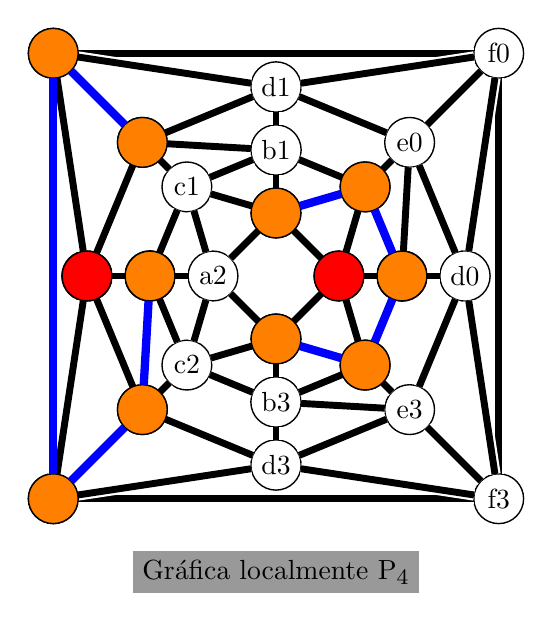
\begin{tikzpicture}[scale=0.8]
      \grCycle[RA=1,prefix=a]{4}
      \grEmptyCycle[RA=2,prefix=b]{4}
      \grEmptyCycle[RA=3,prefix=d]{4}
      \begin{scope}[rotate=45]
        \grEmptyCycle[RA=2,prefix=c]{4}
        \grEmptyCycle[RA=3,prefix=e]{4}
        \grCycle[RA=5,prefix=f]{4}
      \end{scope}
      \EdgeIdentity{b}{a}{4}
      \EdgeIdentity{b}{c}{4}
      \EdgeIdentity{b}{e}{4}
      \EdgeIdentity{a}{c}{4}
      \EdgeIdentity{b}{d}{4}
      \EdgeIdentity{d}{e}{4}
      \EdgeIdentity{c}{e}{4}
      \EdgeIdentity{d}{f}{4}
      \EdgeIdentity{e}{f}{4}
      \EdgeMod{c}{b}{4}{1}
      \EdgeMod{e}{d}{4}{1}
      \EdgeMod{f}{d}{4}{1}
      \EdgeMod{a}{c}{4}{3}
      \uncover<2-4>{\AddVertexColor{red}{a0}}
      \uncover<3-4>{\AddVertexColor{orange}{a3,c3,b0,c0,a1}}
      \uncover<4>{{%
          \SetUpEdge[lw=3pt,color=blue]
          \Edge(a3)(c3)
          \Edge(b0)(c3)
          \Edge(b0)(c0)
          \Edge(c0)(a1)
        }}
      \uncover<5-7>{\AddVertexColor{red}{d2}}
      \uncover<6-7>{\AddVertexColor{orange}{b2,e2,f2,f1,e1}}
      \uncover<7>{{%
          \SetUpEdge[lw=3pt,color=blue]
          \Edge(b2)(e2)
          \Edge(e2)(f2)
          \Edge(f2)(f1)
          \Edge(f1)(e1)
          }}
      \uncover<8>{\graphcaption{0}{-4.7}{Gráfica localmente $P_{4}$}}
    \end{tikzpicture}
  \end{center}  
\end{standaloneframe}
\end{document}
